\subsubsection{Sphere}
The simplest body one can specify is a sphere. The body's section is opened by \lstinline{[sphere: NAME]}. Its size is determined by a  vector pointing from the sphere's center (at the origin of the coordinate system) to an arbitrary point on its surface.

\paragraph{Parameters}
\begin{description}
 \item{\lstinline{radius_vector}} Vector whose length specifies the sphere's radius.
\end{description}

\paragraph{Example}\ 

\lstinputlisting{srcexamples/sphere.ini}
\ \\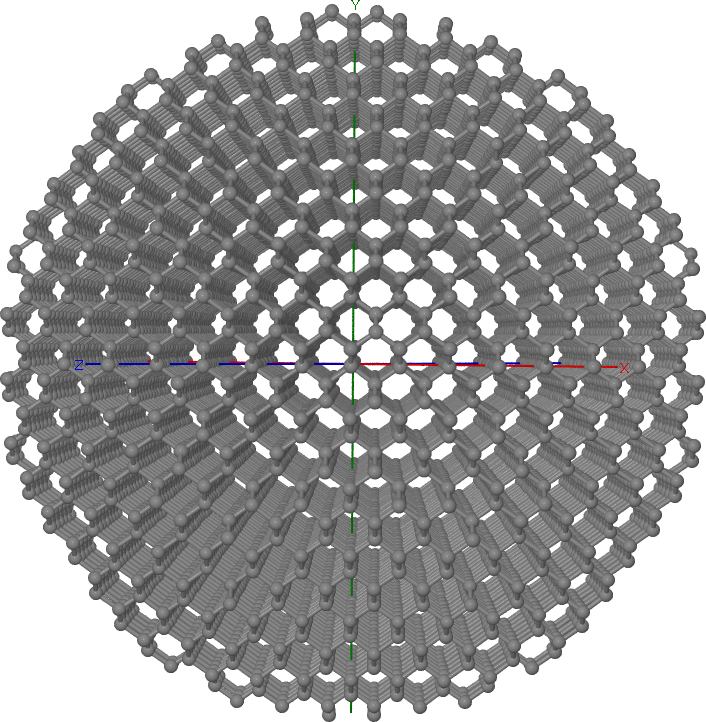
\includegraphics[width=0.6\textwidth]{srcexamples/sphere.png}